%!TEX root=Principal.tex
\chapter{TABELAS DE PROBABILIDADES CONDICIONAIS}
\label{ap:tpc}

\begin{figure}[ht!]
    \centering
    \begin{minipage}{\textwidth}
        \caption{TPC - alfredo}
        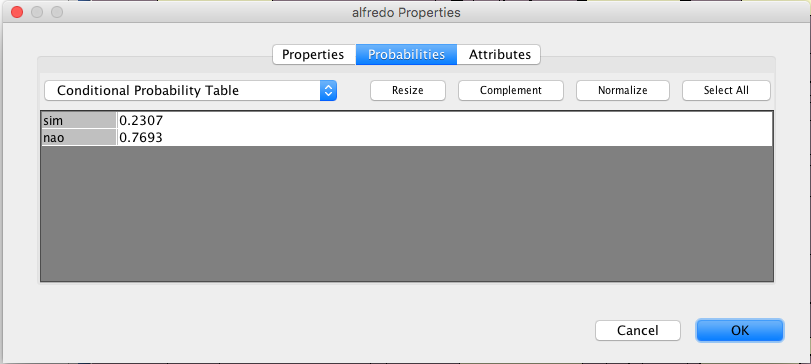
\includegraphics[width=\textwidth]{tpc_alfredo}
        \smallcaption{Fonte: Autor.}
    \end{minipage}
\end{figure}

\begin{figure}[ht!]
    \centering
    \begin{minipage}{\textwidth}
        \caption{TPC - maria\_eduarda}
        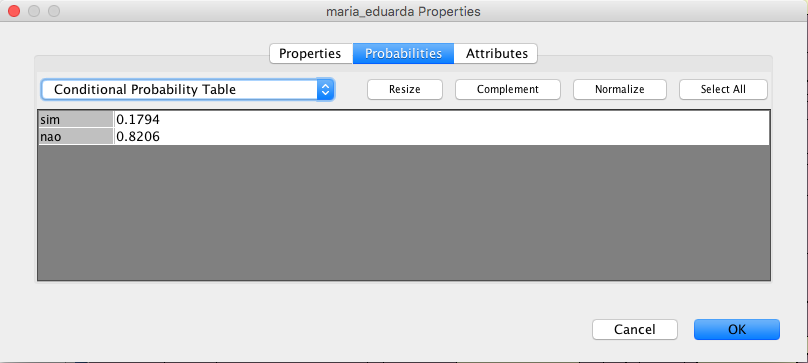
\includegraphics[width=\textwidth]{tpc_maria_eduarda}
        \smallcaption{Fonte: Autor.}
    \end{minipage}
\end{figure}

\begin{figure}[ht!]
    \centering
    \begin{minipage}{\textwidth}
        \caption{TPC - manuel}
        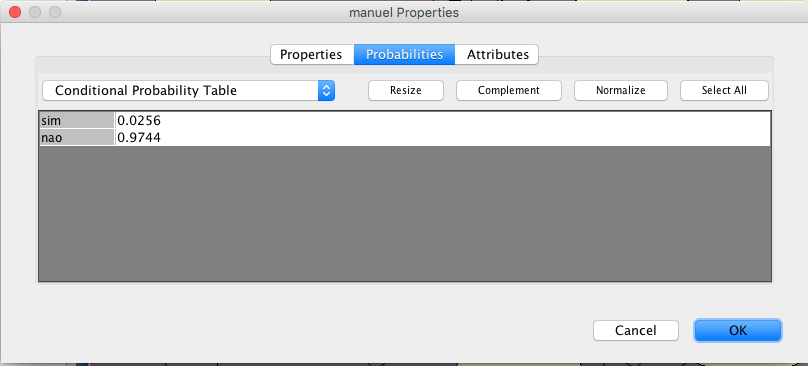
\includegraphics[width=\textwidth]{tpc_manuel}
        \smallcaption{Fonte: Autor.}
    \end{minipage}
\end{figure}

\begin{figure}[ht!]
    \centering
    \begin{minipage}{\textwidth}
        \caption{TPC - danielo}
        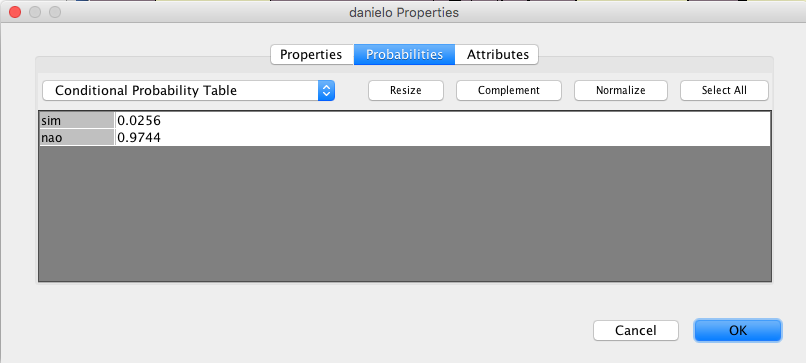
\includegraphics[width=\textwidth]{tpc_danielo}
        \smallcaption{Fonte: Autor.}
    \end{minipage}
\end{figure}

\begin{figure}[ht!]
    \centering
    \begin{minipage}{\textwidth}
        \caption{TPC - joaquim}
        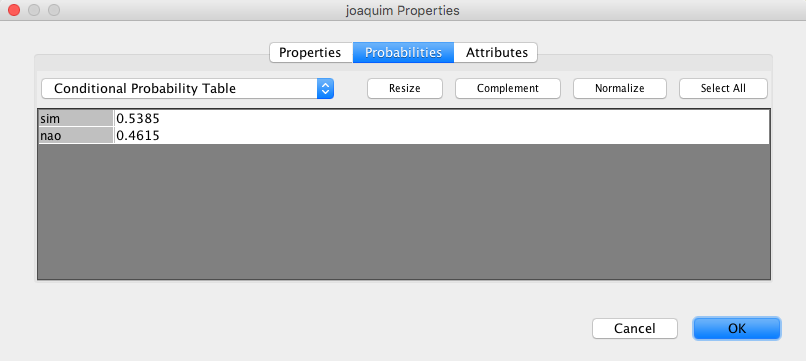
\includegraphics[width=\textwidth]{tpc_joaquim}
        \smallcaption{Fonte: Autor.}
    \end{minipage}
\end{figure}

\begin{figure}[ht!]
    \centering
    \begin{minipage}{\textwidth}
        \caption{TPC - ajuda}
        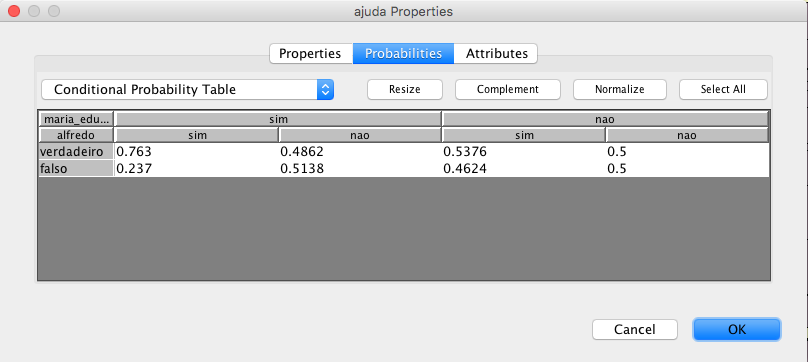
\includegraphics[width=\textwidth]{tpc_ajuda}
        \smallcaption{Fonte: Autor.}
    \end{minipage}
\end{figure}

\begin{figure}[ht!]
    \centering
    \begin{minipage}{\textwidth}
        \caption{TPC - face}
        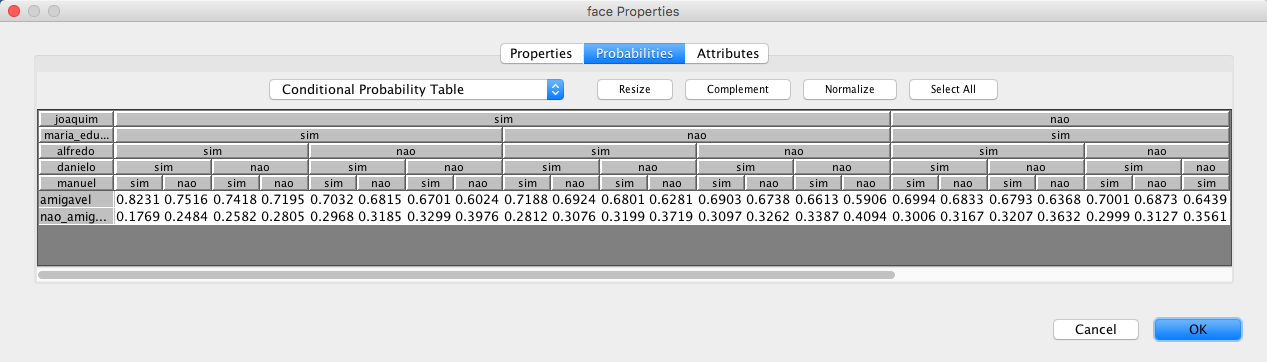
\includegraphics[width=\textwidth]{tpc_face_p1}
        \smallcaption{Fonte: Autor.}
    \end{minipage}
\end{figure}

\begin{figure}[ht!]
    \centering
    \begin{minipage}{\textwidth}
        \caption{TPC - face}
        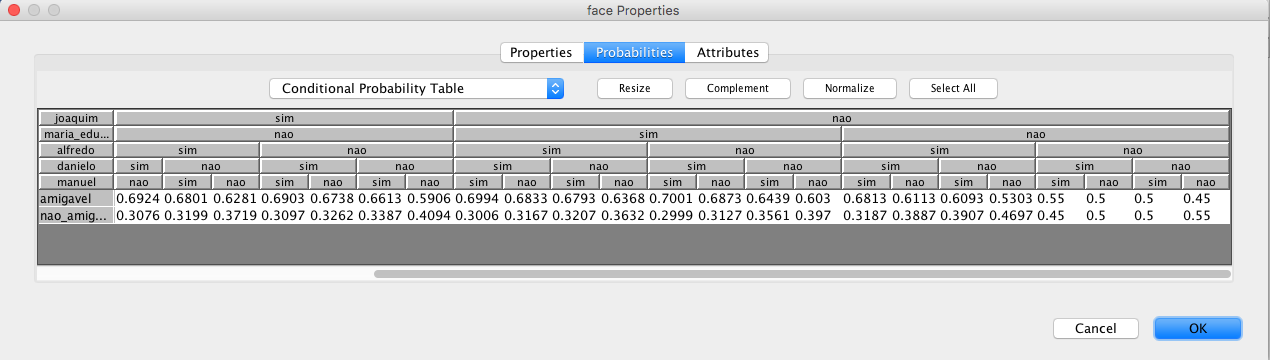
\includegraphics[width=\textwidth]{tpc_face_p2}
        \smallcaption{Fonte: Autor.}
    \end{minipage}
\end{figure}

\begin{figure}[ht!]
    \centering
    \begin{minipage}{\textwidth}
        \caption{TPC - fala}
        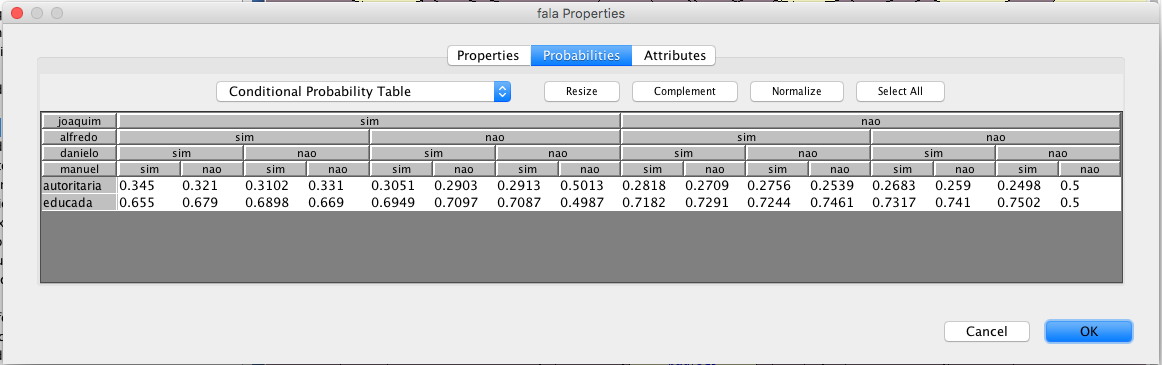
\includegraphics[width=\textwidth]{tpc_fala}
        \smallcaption{Fonte: Autor.}
    \end{minipage}
\end{figure}

\begin{figure}[ht!]
    \centering
    \begin{minipage}{\textwidth}
        \caption{TPC - feedback}
        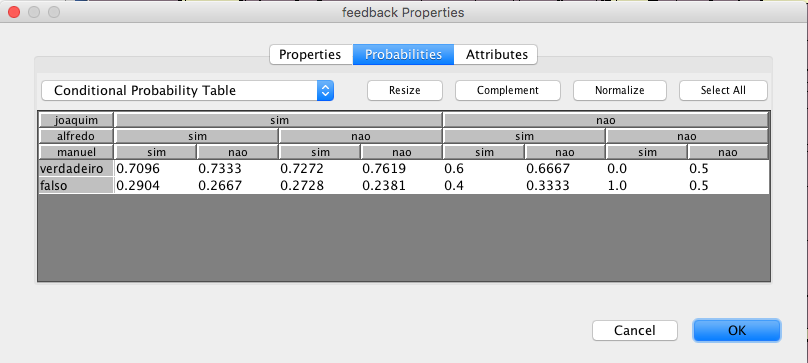
\includegraphics[width=\textwidth]{tpc_feedback}
        \smallcaption{Fonte: Autor.}
    \end{minipage}
\end{figure}

\begin{figure}[ht!]
    \centering
    \begin{minipage}{\textwidth}
        \caption{TPC - gestos}
        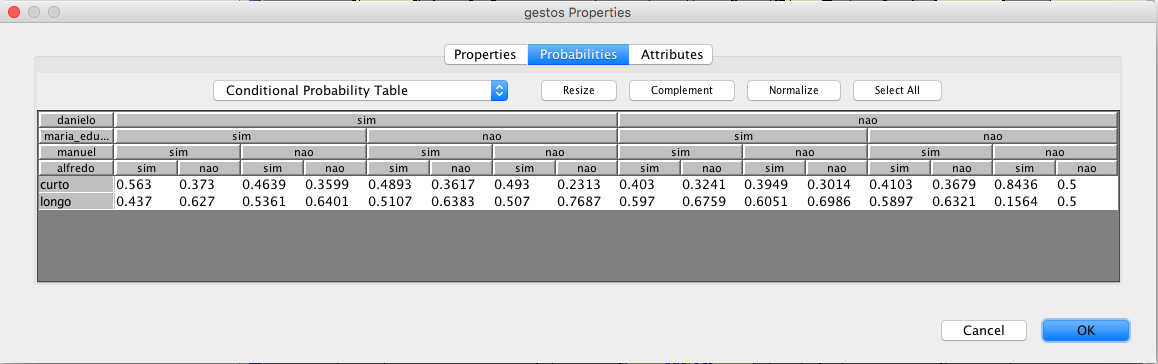
\includegraphics[width=\textwidth]{tpc_gestos}
        \smallcaption{Fonte: Autor.}
    \end{minipage}
\end{figure}

\begin{figure}[ht!]
    \centering
    \begin{minipage}{\textwidth}
        \caption{TPC - padroes}
        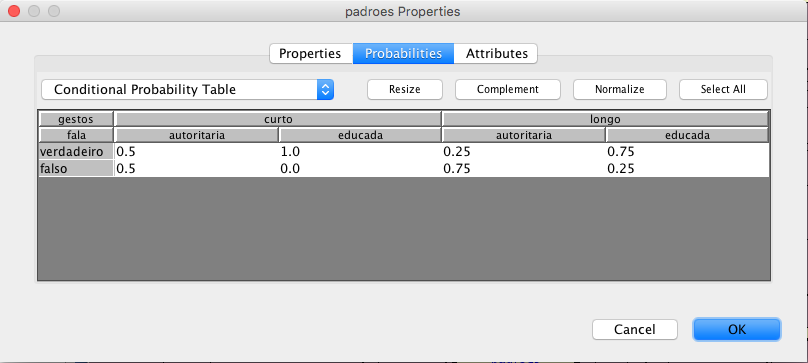
\includegraphics[width=\textwidth]{tpc_padroes}
        \smallcaption{Fonte: Autor.}
    \end{minipage}
\end{figure}

\begin{figure}[ht!]
    \centering
    \begin{minipage}{\textwidth}
        \caption{TPC - posicao}
        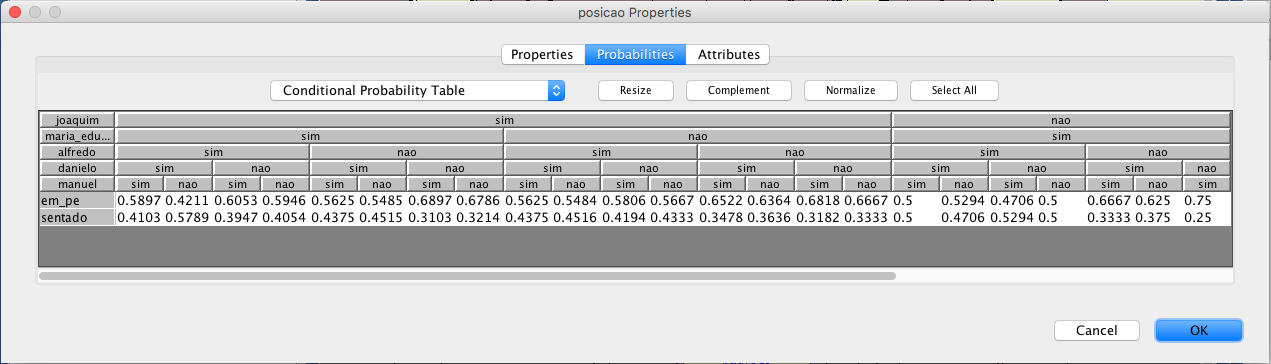
\includegraphics[width=\textwidth]{tpc_posicao_p1}
        \smallcaption{Fonte: Autor.}
    \end{minipage}
\end{figure}

\begin{figure}[ht!]
    \centering
    \begin{minipage}{\textwidth}
        \caption{TPC - posicao}
        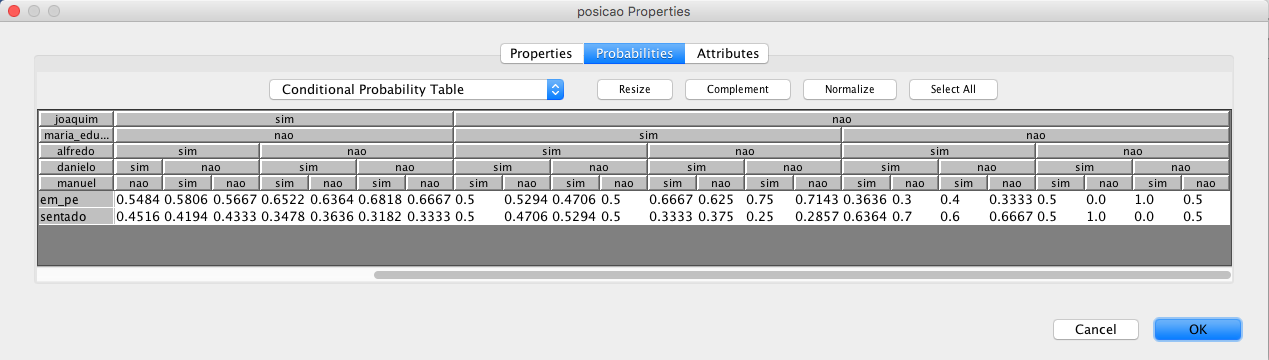
\includegraphics[width=\textwidth]{tpc_posicao_p2}
        \smallcaption{Fonte: Autor.}
    \end{minipage}
\end{figure}

\begin{figure}[ht!]
    \centering
    \begin{minipage}{\textwidth}
        \caption{TPC - proximidade}
        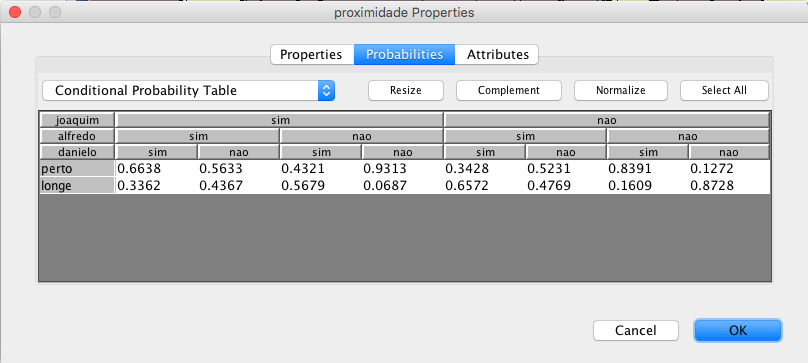
\includegraphics[width=\textwidth]{tpc_proximidade}
        \smallcaption{Fonte: Autor.}
    \end{minipage}
\end{figure}

\begin{figure}[ht!]
    \centering
    \begin{minipage}{\textwidth}
        \caption{TPC - reconhecer}
        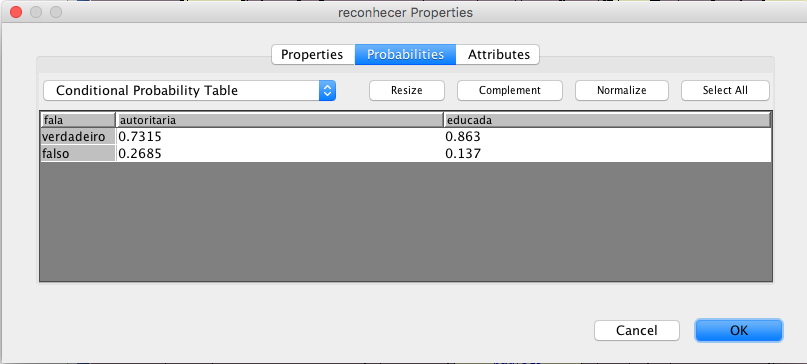
\includegraphics[width=\textwidth]{tpc_reconhecer}
        \smallcaption{Fonte: Autor.}
    \end{minipage}
\end{figure}

\begin{figure}[ht!]
    \centering
    \begin{minipage}{\textwidth}
        \caption{TPC - toque}
        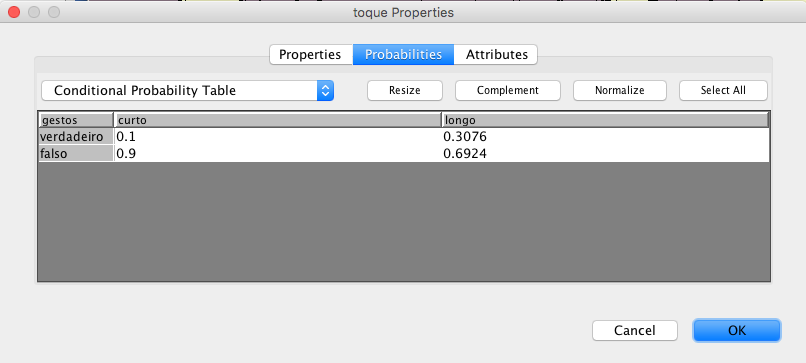
\includegraphics[width=\textwidth]{tpc_toque}
        \smallcaption{Fonte: Autor.}
    \end{minipage}
\end{figure}

\begin{figure}[ht!]
    \centering
    \begin{minipage}{\textwidth}
        \caption{TPC - velocidade}
        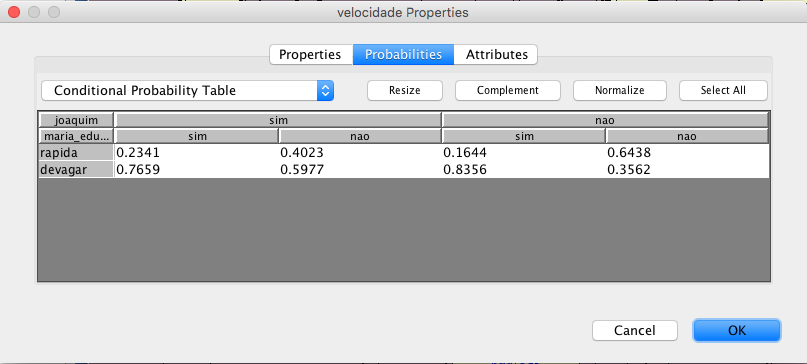
\includegraphics[width=\textwidth]{tpc_velocidade}
        \smallcaption{Fonte: Autor.}
    \end{minipage}
\end{figure}

\begin{figure}[ht!]
    \centering
    \begin{minipage}{\textwidth}
        \caption{TPC - conforto}
        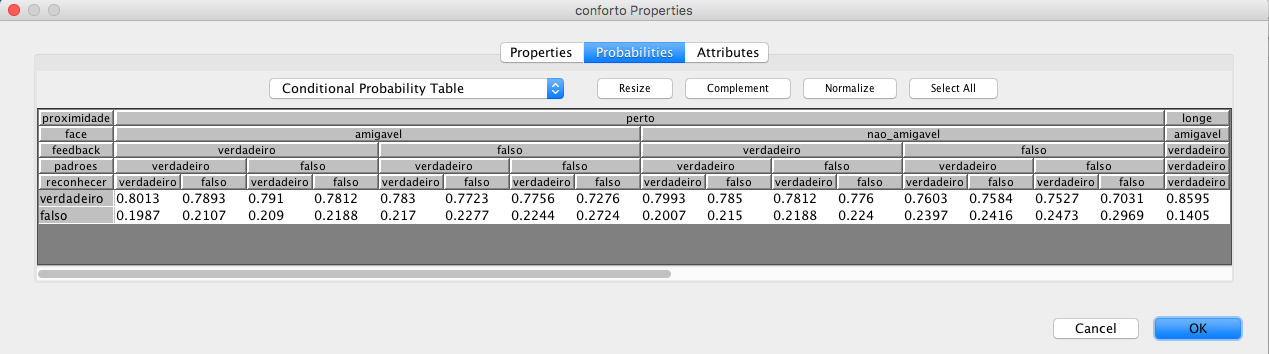
\includegraphics[width=\textwidth]{tpc_conforto_p1}
        \smallcaption{Fonte: Autor.}
    \end{minipage}
\end{figure}

\begin{figure}[ht!]
    \centering
    \begin{minipage}{\textwidth}
        \caption{TPC - conforto}
        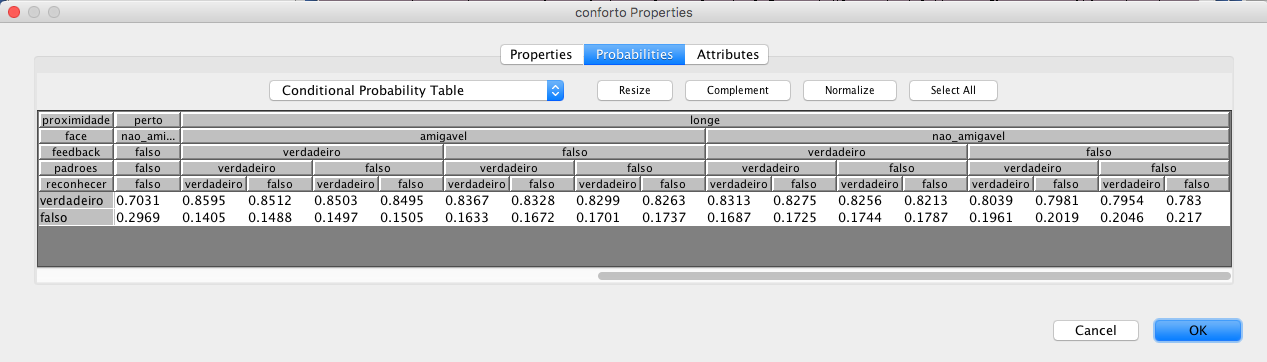
\includegraphics[width=\textwidth]{tpc_conforto_p2}
        \smallcaption{Fonte: Autor.}
    \end{minipage}
\end{figure}

\begin{figure}[ht!]
    \centering
    \begin{minipage}{\textwidth}
        \caption{TPC - desconforto}
        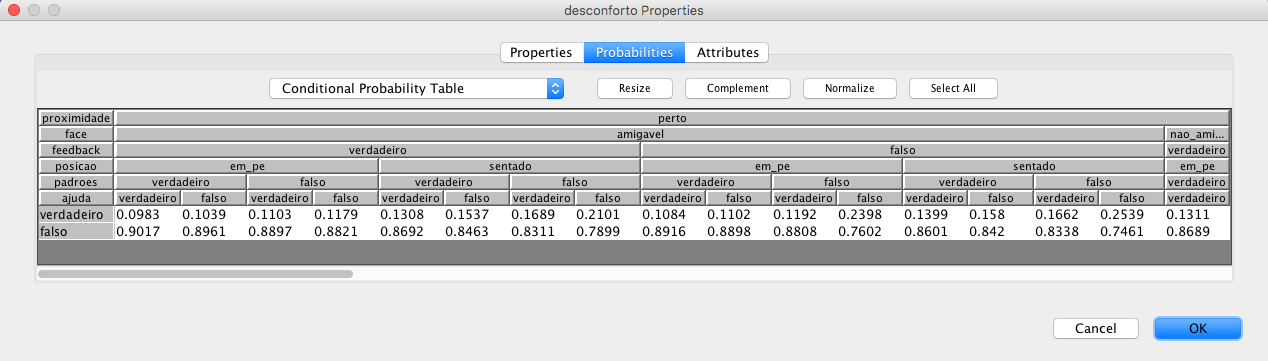
\includegraphics[width=\textwidth]{tpc_desconforto_p1}
        \smallcaption{Fonte: Autor.}
    \end{minipage}
\end{figure}

\begin{figure}[ht!]
    \centering
    \begin{minipage}{\textwidth}
        \caption{TPC - desconforto}
        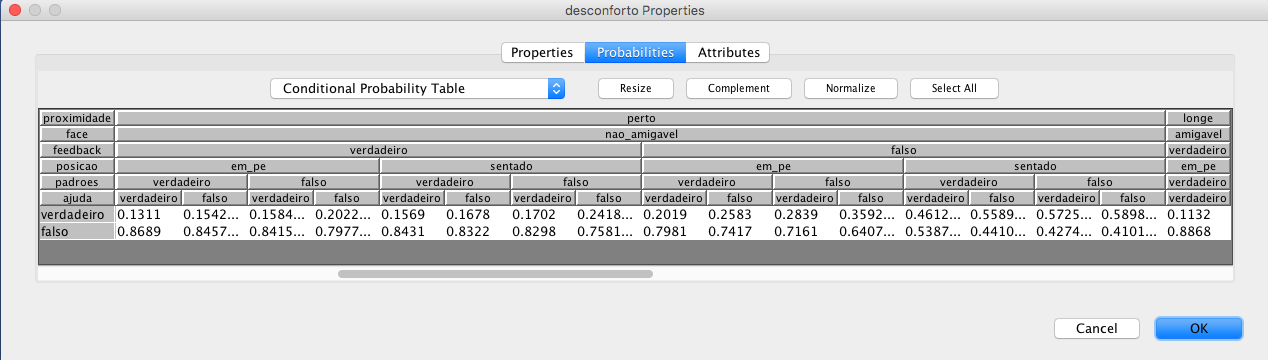
\includegraphics[width=\textwidth]{tpc_desconforto_p2}
        \smallcaption{Fonte: Autor.}
    \end{minipage}
\end{figure}

\begin{figure}[ht!]
    \centering
    \begin{minipage}{\textwidth}
        \caption{TPC - desconforto}
        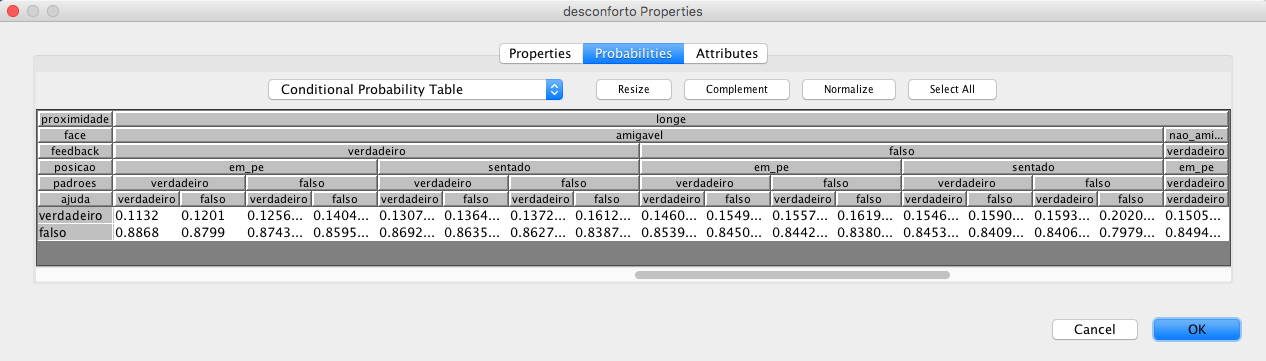
\includegraphics[width=\textwidth]{tpc_desconforto_p3}
        \smallcaption{Fonte: Autor.}
    \end{minipage}
\end{figure}

\begin{figure}[ht!]
    \centering
    \begin{minipage}{\textwidth}
        \caption{TPC - desconforto}
        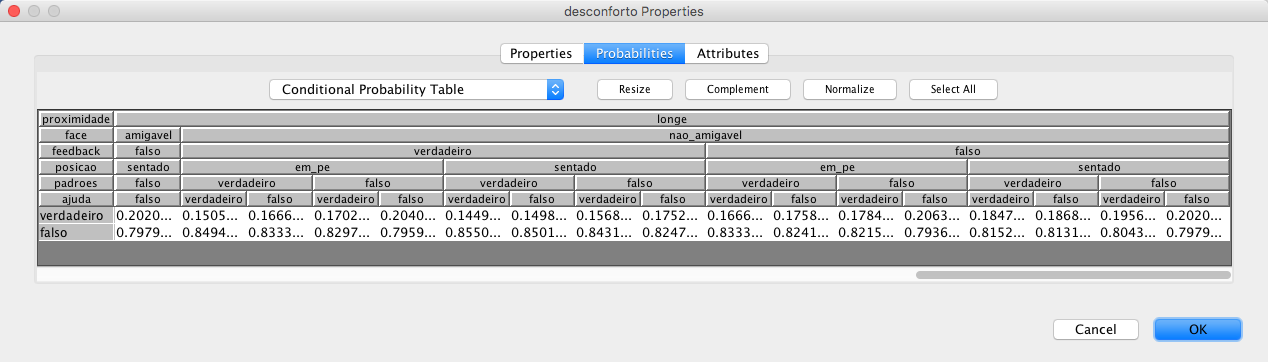
\includegraphics[width=\textwidth]{tpc_desconforto_p4}
        \smallcaption{Fonte: Autor.}
    \end{minipage}
\end{figure}

\begin{figure}[ht!]
    \centering
    \begin{minipage}{\textwidth}
        \caption{TPC - medo}
        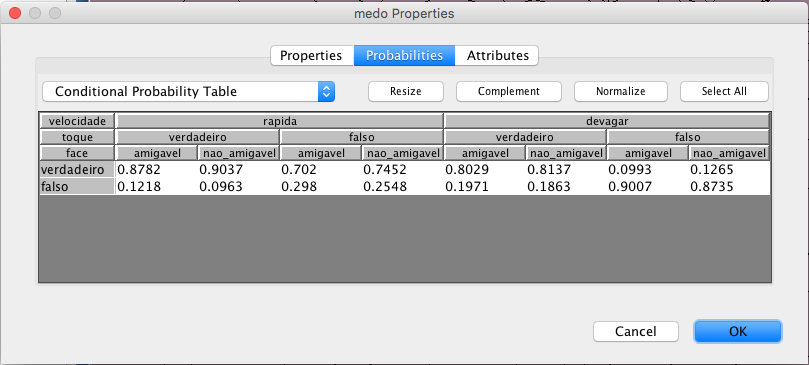
\includegraphics[width=\textwidth]{tpc_medo}
        \smallcaption{Fonte: Autor.}
    \end{minipage}
\end{figure}